%---------Definición de paquetes base--------------
\documentclass[12pt,letterpaper]{article}
\usepackage[utf8]{inputenc}
\usepackage{amsmath}
\usepackage{amsfonts}
\usepackage{amssymb}
\usepackage{url}
\usepackage{graphicx} 
\usepackage{float}
\usepackage{enumitem}
\usepackage{tabularx}
\usepackage{booktabs} % Required for nicer horizontal rules in tables
\usepackage[spanish, es-tabla, es-nodecimaldot]{babel}		%Separacion silabica espanola
\usepackage[left=2.00cm, right=2.00cm, top=2.00cm, bottom=2.00cm]{geometry}
\usepackage{multicol}	% Para manejar columnas múltiples
\usepackage{longtable}  % Para manejar tablas de varias paginas con encabezado
		\newenvironment{Table}
		{\par\medskip\noindent\minipage{\linewidth}}
		{\endminipage\par\medskip}
\usepackage{fancyhdr}	% Para manejar los encabezados y pies de pagina
		\pagestyle{fancy}		% Contenido de los encabezados y pies de pagina
\usepackage{wrapfig}	% Necesario para la rubrica de evaluación
%--------Encabezado y pie de página---------------------
\lhead{Computacional I}
\chead{}
\rhead{Evaluación 2}	% va el numero de experimento, al igual que en el titulo
\lfoot{Lic. en Física}
\cfoot{\thepage\ }
\rfoot{Universidad de Sonora}
%-----------Portada---------------------------------------------
\author{
Leonardo Coronado Arvayo\\
Profesor: Carlos Lizárraga Celaya   \vspace*{1.25in}}
\title{	\includegraphics[width=3cm]{Logo} \\
Universidad de Sonora \\
{\small Departamento de Física \\
Licenciatura en Física \\
Computacional I \\
2017-1 \\
\vspace{0.55in} Reporte}\\ 
{\Huge Evaluación \#2: Manchas solares y Fourier}\\
\vspace*{1.0in}}
%-----------Reporte----------------------------
%	Portada y tabla de contenidos
\begin{document}
	\pagenumbering{gobble} % Remove page numbers (and reset to 1)
	\maketitle
\newpage
	\pagenumbering{arabic}


\section{Preguntas}

\begin{itemize}

\item De los datos proporcionados, utiliza una transformada discreta de Fourier, para encontrar la frecuencia del ciclo principal. Muestra una gráfica con los principales modos encontrados.  

\begin{table}[H]
\centering
\begin{tabular}{|c|ccc|}

\hline
Amplitud	&	n	&	Periodo en meses & Periodo en años\\
33.72 & 1.93 & 136.60 & 11.38 \\
\hline 

\end{tabular}
\caption{Características del nodo principal}
\end{table}

 \begin{figure}[H]
	\centering
	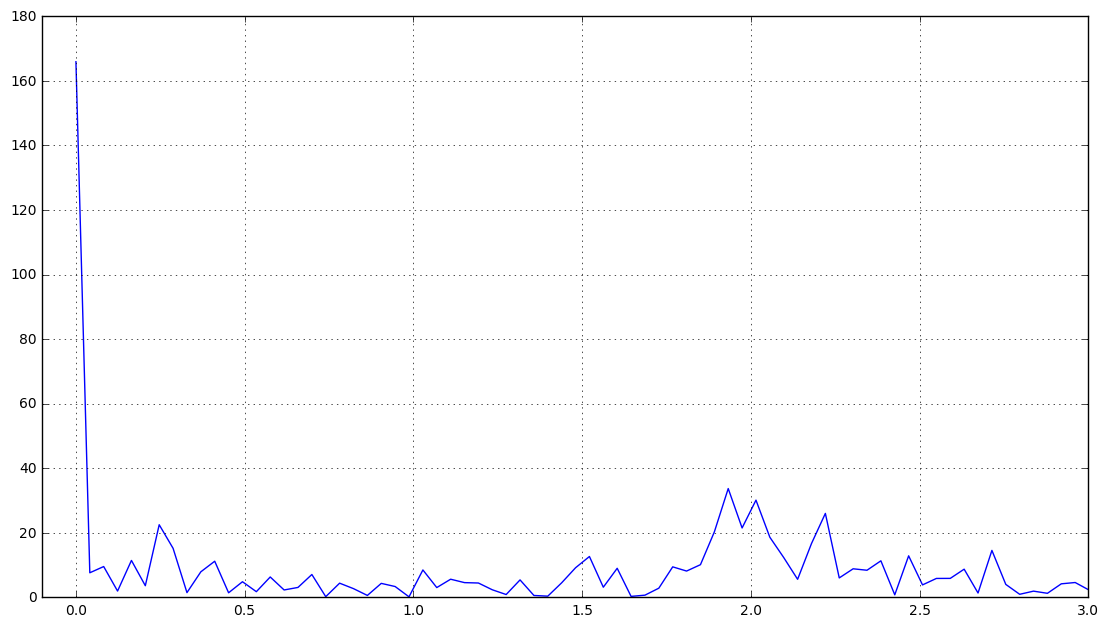
\includegraphics[height=9cm]{four}
	\caption{Principales nodos para las manchas solares}
\end{figure}

\item ¿Encuentras un solo ciclo principal o un conjunto de ciclos con frecuencia cercana? ¿Cuál sería el promedio del conjunto de frecuencias?

Los principales 3 periodos tienen una frecuencia cercana. El promedio $P_{frecuencias}$ esta dado como:
$$ P_{frecuencias} = \frac{f_{1}+f_{2}+f_{3}}{3}= \frac{11.38+10.92+9.91}{3} = 10.74   \ a\tilde nos$$

Entonces el promedio del conjunto de las frecuencias es de 10.74 años.

\item ¿Que otros ciclos relevantes encuentras? Proporciona una tabla con las amplitudes de los ciclos. 

\begin{table}[H]
\centering
\begin{tabular}{|c|cc|}

\hline
Amplitud	&	n	&	 Periodo en años\\
\hline
33.72 & 1.93  & 11.38 \\
30.13 & 2.01 & 10.92 \\
26.02 & 2.22 & 9.91 \\
21.52 & 1.97 & 11.15\\
20.29 & 1.89 & 11.63\\
14.57 &2.06  &  10.69 \\
15.21 & 2.17 &  10.09\\
\hline 

\end{tabular}
\caption{Características de los nodos principales}
\end{table}

El promedio de estos 10 principales nodos salio de 10.83 años.

\item Lo que han encontrado hasta ahora son ciertas regularidades, incluso hay pronósticos de un rango para el número de manchas solares. ¿Cómo crees que es posible predecir el número de manchas?

No estoy muy seguro de entender la pregunta pero me imagino que seria posible predecir el numero de manchas por ciclo aplicando un ajuste de Fourier aunque no se si sea necesario hacerlo ciclo por ciclo, en lugar de todo el periodo.


\end{itemize}
   



\end{document}